%!TEX root = main.tex

\newpage
\subsection{수식 작성하기}
드디어 \lt 의 꽃, 수식에 대해 설명을 드릴 차례입니다.
다른 어떤 편집기보다도 강력하고 편리한 수식 편집 기능을 가지고 있는 \lt 인 만큼, 실질적으로 수식 편집의 표준으로 자리 잡았기 때문에 다양한 곳에서 이제 배우는 것들을 이용할 수 있을 겁니다.
역시나 예시부터 볼까요?

\begin{Verbatim}[frame=single]
\documentclass{article}
\usepackage{kotex}
\usepackage{setspace}
\usepackage{amsmath}
\usepackage{amssymb}
\usepackage[left=2.5cm,right=2.5cm,top=3cm,bottom=3cm,a4paper]{geometry}
\begin{document}
	\doublespacing
	\noindent 수식을 입력해 봅시다.\\
	막 내용을 입력하다 중간에 짧은 수식을 넣을 수 있습니다.\\
	예를 들어 $c \in A$ 이렇게 말입니다.\\
	조금 길거나 큰 수식을 따로 입력할 수도 있습니다.\\
	예를 들어
	\[\left\{ \begin{array}{ll}
		a \in f(a)
		\\a \notin f(a)
	\end{array} \right.\]
	이렇게 말입니다.\\
	심지어
	\begin{align}
		|f(x)|=|sf_1(x)+tf_2(x)| &\le |sf_1(x)|+|tf_2(x)| \nonumber
		\\&=|s||f_1(x)|+|t||f_2(x)| \nonumber
		\\&\le |s|c_1|g(x)|+|t|c_2|g(x)| \nonumber
		\\&=(|s|c_1+|t|c_2)|g(x)| \nonumber
	\end{align}
	이런 것도 됩니다.\\
	\LaTeX 은 정말 많은 수식 요소들을 지원해줍니다.\\
	$a^{bcd}_{efg}$와 같은 첨자는 물론이고, $\sum$, $\int$같은 것도 지원합니다.
	\[\frac{\pi}{2}\]
	이렇게 분수도 잘 됩니다.
\end{document}
\end{Verbatim}
역시 바로 다음 페이지에서 결과물을 확인하실 수 있습니다.

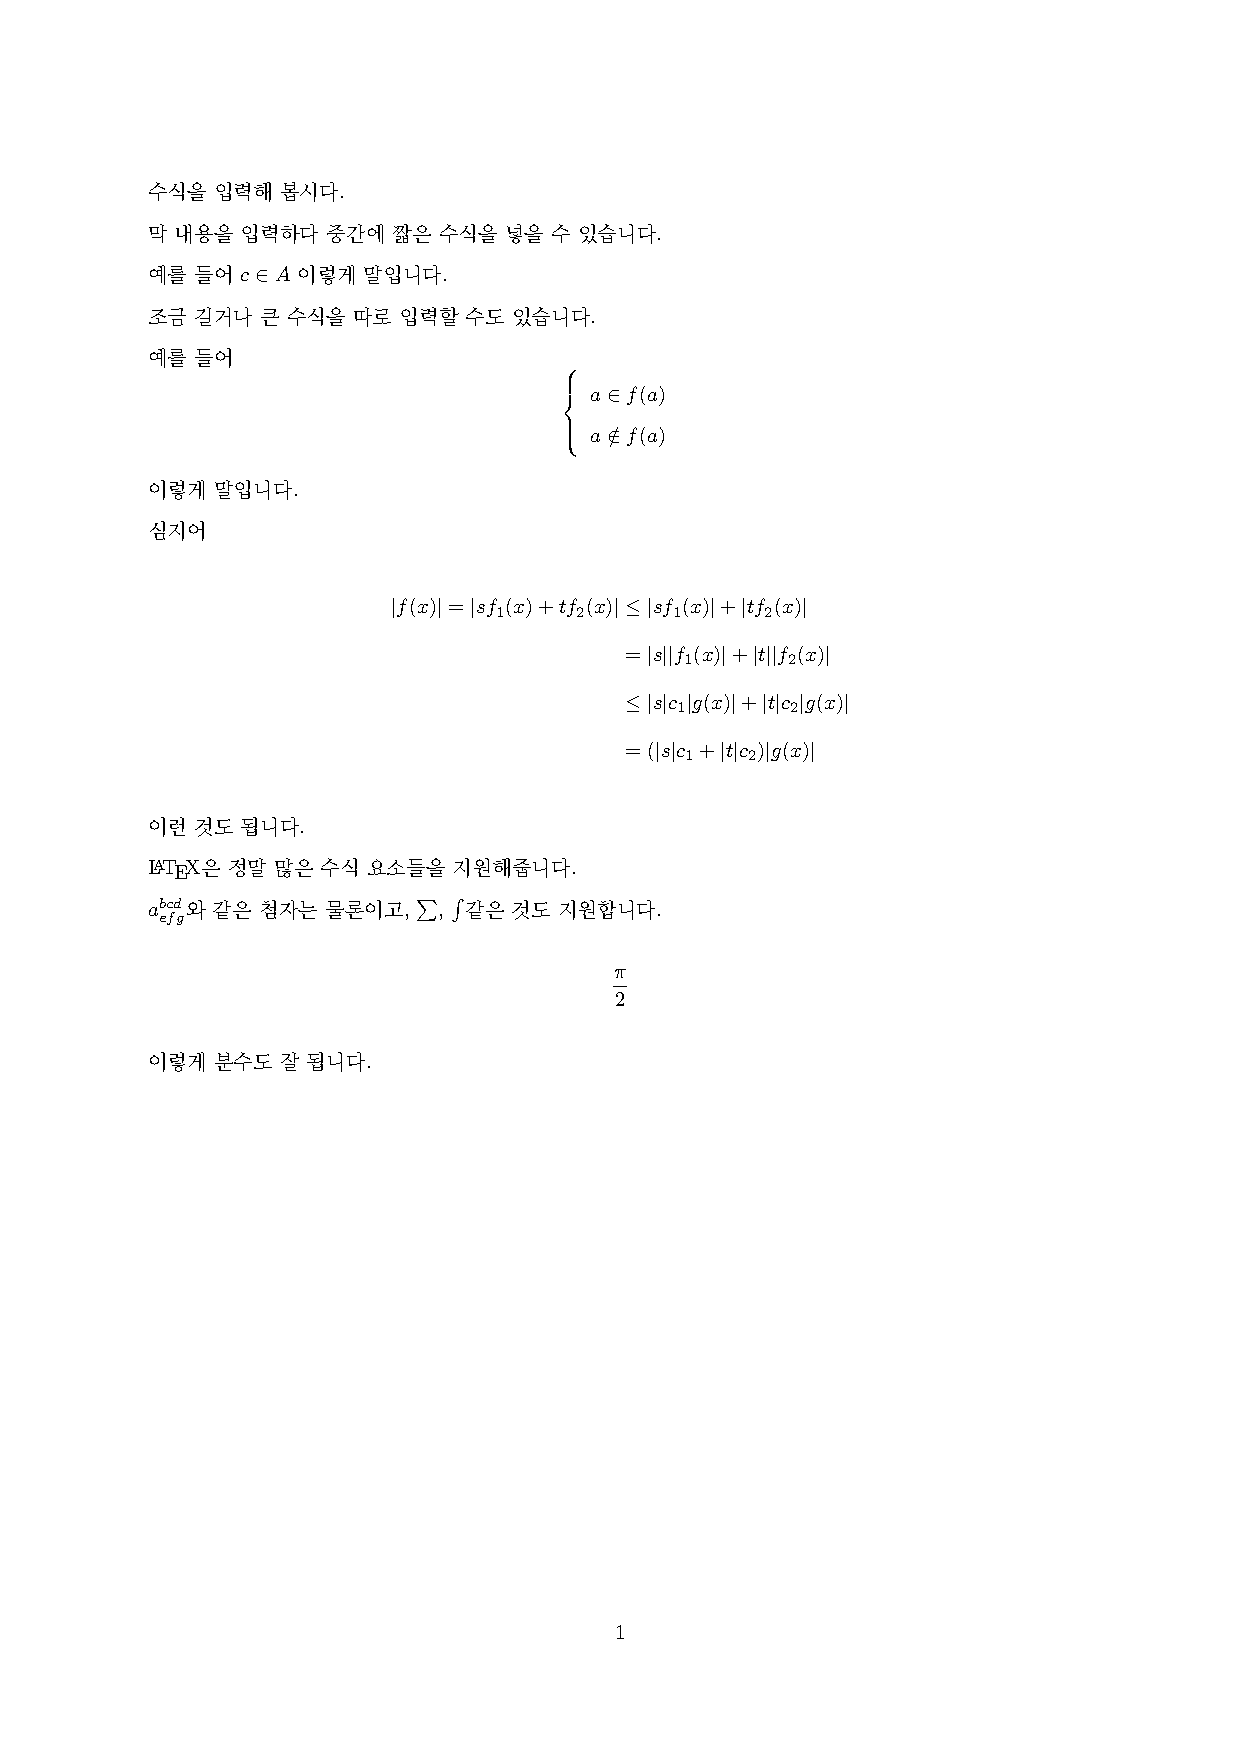
\includepdf[fitpaper=true]{example/mathexamplepdf.pdf}

\subsubsection{입력 시작하기}
\lt 에서 수식을 입력하기 위해서는 따로 수식 편집기를 킨다거나, 그림을 추가하듯 추가하는 것이 아니라 기호 또는 command를 통해 수식을 입력함을 표시하면 됩니다.
그 방식에는 크게 세 가지 정도가 있습니다.

\paragraph{짧은 수식 삽입하기}
길고 크고 엄청난 수식을 입력하는 것이 아니라면, 보통의 경우는 수식을 문장의 중간에 넣고 싶을 겁니다.
이 때에는 내용을 입력하다가 수식을 입력하고 싶을 때 \verb|$ \dots $|를 이용하면 됩니다.

%%% Local Variables:
%%% mode: latex
%%% TeX-master: "main"
%%% End:
